\documentclass[12pt]{article}

% custom commands
\newcommand{\paren}[1]{\left( {#1} \right)}
\newcommand{\abs}[1]{\left| {#1} \right|}

% Math and symbol packages
\usepackage{amsmath}
\usepackage{amssymb}
\usepackage{derivative}

% Figure Packages
\usepackage{graphicx}
\usepackage{wrapfig}
\usepackage{epstopdf}
\usepackage{float}
\usepackage{subfigure}

% Formatting and Random Text Generation
\usepackage{inputenc}
\usepackage[left=2.54cm,right=2.54cm,top=2.54cm,bottom=2.54cm]{geometry}
\usepackage{lipsum}

% Header and indent packages
\usepackage{fancyhdr}
\usepackage{indentfirst}

% Create Title Section
\title{Charge to Mass Ratio of the Electron \\ \small (EOM)}
\author{Trevor Swan \\
Department of Physics, Case Western Reserve University \\
Cleveland, OH 44016-7079}
\date{2/25/25}

% Create paragraph formatting
%\setlength{\parindent}{3em}

% Actual Lab content
\begin{document}
\pagestyle{fancy}
\fancyhf{}

% Load the title
\maketitle
\thispagestyle{fancy}
\renewcommand{\headrulewidth}{0pt}

% Set up Footers
\fancyfoot[L]{Trevor Swan}
\fancyfoot[C]{\thepage}
\fancyfoot[R]{Charge to Mass Ratio of the Electron}

% Abstract section of Report
\section{Abstract}
I have tested the electron to mass ratio for a commercial apparatus using principles of electromagnetism. Using Helmholtz coils and two power supplies, along with linear regression analysis of experimental parameters, I have determined two numerical values for $\frac{e}{m}$. For the first value, a constant voltage of $V=104\pm1V$ was applied through the apparatus with varied current, which yielded a charge to mass ratio of $5.5\times10^{14}\pm1.2\times10^{18} \frac{C}{Kg}$. In this experiment, 5 beam radii were determined from 5 roughly evenly spaced current values, ranging from 0.66A to 1.91A. For the second value, a constant current of $A=1.02A\pm0.1A$ was applied through the apparatus with varied voltage, which yielded a ratio of $1.1\times10^{15}\pm2.6\times10^{14} \frac{C}{Kg}$. In this experiment, 5 beam radii were determined from 5 roughly evenly spaced voltage values, ranging from 84V to 197V. The latter reported value was chosen as the concluding value, despite deviating from the expected CODATA value of $\frac{e}{m}=(1.75882017\pm0.00000007)\times10^{11} \frac{C}{Kg}$. This discrepancy, while less severe than the first reported value, is still quite large. It can be expected, however, that there will be much less precision from shared equipment during a 1.5 hour time frame compared to a professional and critically measured value. This discrepancy is most likely a result of systematic error, where the coils and power supplies used were most likely marginally inaccurate or inconsistent, and other students in the room contributed to stray magnetic fields. Systematic errors were littered throughout this experiment, negatively impacting calculations and preventing strong conclusions.

% Introduction and Thoery
\section{Introduction and Theory}
An electron moving with a given velocity $\vec{v}$ in an applied magnetic field $\vec{B}$ is influenced by a force know as the Lorentz force, given by

\begin{equation}
	\vec{F} = -e\paren{\vec{v}\times\vec{B}} \label{e:Lorentz}
\end{equation}

Due to the nature of this electric force, whose magnitude is $evB$, the electron travels along a circular path with a radius $R$. As the Lorentz for acts centripetally, the acceleration of the electron is $\frac{v^2}{R}$. Thus, we can apply Newton's Second Law and some basic algebraic manipulations to yield the expression

\begin{equation}
	evB=\frac{mv^2}{R}\rightarrow \frac{e}{m}=\frac{2V}{(BR)^2}
	\label{e:N2L_e_over_m}
\end{equation}

According to CODATA's recommended value~(\ref{ref:MANUEL}), we expect to measure a value for $\frac{e}{m}$ close to

\begin{equation*}
	\frac{e}{m}=(1.75882017\pm0.00000007)\times10^{11} \frac{C}{Kg}
\end{equation*} 

As explained in the following section, this experiment makes use of a Helmholtz coil that provides a uniform magnetic field perpendicular to the electron beam, inline with the conditions for the previous derivations. The field at the center of this field is given by the equation

\begin{equation}
	B=\frac{8\mu_0NI_c}{5r\sqrt{5}} \label{e:Helmholtz_field}
\end{equation}

\noindent where $\mu_0=4\pi\times10^{-7} \frac{T\cdot m}{A}$, $I_c$ is the current in the coil, N is the number of turns in the coil, and r is the radii of the coil. Values for the coil's constants are discussed in the following section. To alter the electron trajectory, $I_c$ can be changed to influence the magnetic field $B$, or different voltage values can be applied.

Combining the simplified expression from Equation \ref{e:N2L_e_over_m} with Equation \ref{e:Helmholtz_field}, $B$ can be eliminated from the expression yielding

\begin{equation}
	\frac{e}{m}=\frac{2V}{\paren{\frac{8\mu_0N}{5r\sqrt{5}}}^2I_c^2R^2} \label{e:em_full_expr}
\end{equation}

\noindent This equation can be used to show the dependence of $R$ on either $I_c$ or $V$, both of which will be analyzed in this paper.

Due to the nature of voltage and amps, and how they relate to the electrons, we expect to see the beam's radius decrease with increased current at a constant voltage, and the beam's radius increase with increased voltage at a constant current. This is because the radius of the electron beam is dependent on the velocity of the electrons, which can be increased by increasing the energy, or potential difference (Volts).

\subsection{Dependence on Current}

Performing basic algebraic manipulations and defining a proportionality constant $\alpha$, the dependence on the coil current is given by the inverse of the electron beam's radius

\begin{equation}
	\frac{1}{R}=\alpha\cdot I_c \label{e:FixV_dep}
\end{equation}

\noindent where $\alpha$ is given by

\begin{equation}
	\alpha = \frac{8\mu_0N}{5r}\sqrt{\frac{e/m}{10V}} \label{e:FixV_alpha}
\end{equation}

\noindent It should be noted that here, voltage $V$ is constant, or Fixed. Also, $\frac{e}{m}$ is being treated as a constant as well, so that future analysis and regressions can lead to calculating $\frac{e}{m}$ using $\alpha$. Due to residual fields interfering with the $B$-field of the Helmholtz coil, an intercept term $A$ is added to Equation \ref{e:FixV_dep}. In theory, this $A$ value should be equal to 0, but the equipment used is not perfect and thus interference is more than likely. The resulting equation represents a straight line with $\frac{1}{R}$ as the dependent variable, $I_c$ as the independent variable, and $\alpha$ as the slope:

\begin{equation}
	\frac{1}{R}=\alpha I_c + A \label{e:FixV_linear}
\end{equation}

\subsection{Dependence on Voltage}

Conversely, the dependence of $R$, with proportionality constant $\beta$, on the beam voltage can be derived using basic algebraic manipulations as

\begin{equation}
	R=\beta\cdot\sqrt{V} \label{e:FixA_dep}
\end{equation}

\noindent where $\beta$ is given by

\begin{equation}
	\beta=\frac{5r}{8\mu_0NI_c}\sqrt{\frac{10}{\frac{e}{m}}} \label{e:FixA_beta}
\end{equation}

\noindent Similarly, it should be noted that $I_c$ is constant, or fixed, and that $\frac{e}{m}$ is treated as a constant to allow for future analysis through regressions. As done in the fixed voltage model, an intercept $B$ is added to Equation \ref{e:FixA_dep}. In theory, this $B$ value should also be equal to 0, but the equipment used is not perfect and thus interference and inconsistencies in instruments are more than likely. The resulting equation represents a straight line with $R$ as the dependent variable, $\sqrt{V}$ as the independent variable, and $\beta$ as the slope:

\begin{equation}
	R=\beta\cdot\sqrt{V}+\beta \label{e:FixA_linear}
\end{equation}

% Procedure
\section{Experimental Procedure}
Despite varying different aspects of our experiment in the two parts (Voltage and Current), the apparatus used remained the same throughout. Figure \ref{f:EOM_Apparatus} shows the apparatus which is based on a commercial apparatus containing vacuum tube with an electron gun and a small about of helium gas, roughly $10^{-5}$ atmospheres~(\ref{ref:MANUEL}). This tube is designed for measuring the electron's charge to mass ratio $\frac{e}{m}$, and is mounted on a Uchida Chassis. The chassis supports the Helmholtz coils for controlling the magnetic field. These coils each have $N=130$ total turns, and have radii of $r=0.158\pm0.005m$. The Helmholtz coils also have a centimeter ruler mounted on its backside which will be used to make measurements. The current required to operate the Helmholtz current comes from the Elecno power supply shown on the left side of Figure \ref{f:EOM_Apparatus}. This power supply is old and inconsistent, and thus an Ammeter is used to accurately read the current supplied. This is necessary as the Helmholtz coils will be burnt out if the current exceeds 2.0A. The electric potential, or voltage, required to operate the electron gun is provided by the Pasco power supply on the right side of Figure \ref{f:EOM_Apparatus}. This device is relatively accurate (relative to future measurements and calculations), and thus errors in 'meters' reading will not be recorded or mentioned again in this report. Similar to the current limit to protect the Helmholtz coils, the voltage supplied should never exceed 12V. For all voltage adjustments, one should use the '500V' knob, being careful not to make sudden large adjustments in the supplied voltage. To ensure the equipment works properly, we first set our current to 1A and the voltage to 100V. With the lights turned off, we were then able to observe a glowing green ring in the bulb mounted inside the coils. To ensure proper readings in the two upcoming experiments, we then rotated the tube very slightly so that the green ring (the electron trajectories) were circular instead of forming spirals. Once we had aligned the green ring to form a circle, we powered down the power supplies to prepare for the first experiment.

\begin{wrapfigure}{r}{0.5\textwidth}
    \centering
    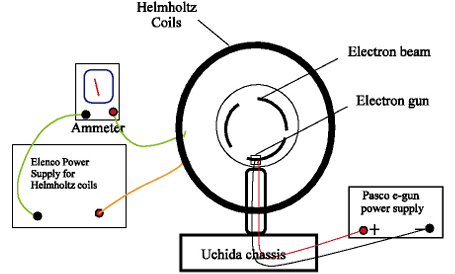
\includegraphics[width=\linewidth]{figures/EOM_Apparatus.png}
    \caption{Experimental Apparatus}
    \label{f:EOM_Apparatus}
\end{wrapfigure}

While adjustments in current/voltage will be discussed in the following subsections, the measurement technique for the electron beam is consistent. When observing the electron beam, the lights in the room must be turned off and you must be aligned with the beam. To eliminate parallax, or the error perceived when viewing two points at an angle~(\ref{ref:MANUEL}), we had to visually align each side of the electron's path with its reflection. To do this, we moved our head back and forth until the reflection of the beam in the mirror mounted at the back of the Helmholtz coils was obscured by the beam itself. At this point each of us would take a measurement, and record it individually in our table. The measured value is the diameter across the entire electron beam. This is because it gives us an easy place to start an end our measurements while providing a convenient way to yield the desired beam radius. We reported our measurements to $0.1 cm$ error, which we believe is representative of the accuracy that can be observed through the apparatus. We would only compare values after both of us took a reading, to prevent collusion. To utilize our data most effectively, we took the average of our measurements. It should be noted that models for this experiment's analysis require data in meters, and thus our average measurements were converted to meters before the final calculation. These values can be seen in Tables \ref{t:FixV} and \ref{t:FixA} on the first two pages of the Appendix.

\subsection{Dependence on Current}
To take measurements and determine the dependence of Current on the beam's radius, we first fixed the Voltage at a value of $104\pm1V$. Then, we found a minimum and maximum current where the beam could be observed. The minimum current corresponded to a value of 0.66A, while the maximum current corresponded to a value of 1.91A. We noted the beam diameter of these current values before proceeding. As expected, the minimum current corresponded to the maximum beam radius, and the maximum current corresponded to the minimum beam size. We then divided the difference of these two extremes by 4 to get a suitable step size of 0.31A, which we then used to record values at 3 intermediate values of current. Such values are reported in Table \ref{t:FixV}. We chose to ignore uncertainties in the error of the varied current, as this experiment assumes current to be a dependent variable whose errors would not be used in a meaningful way in determining $\frac{e}{m}$.

\subsection{Dependence on Voltage}
To take measurements and determine the dependence of Voltage on the beam's radius, we first fixed the current at a value of $1.02\pm0.01A$. Then, we found a minimum and maximum voltage where the beam could be observed. The minimum voltage corresponded to a value of 84V, while the maximum current corresponded to a value of 197V. We noted the beam diameter of these voltage values before proceeding. As theorized, the minimum voltage corresponded to the minimum beam size, and the maximum voltage corresponded to the maximum beam size. We then divided the difference of these two extremes by 4 to get a suitable step size of 28V, which we then used to record values at 3 intermediate values of voltage. Such values are reported in Table \ref{t:FixA}. We chose to ignore uncertainties in the error of the varied voltage, as this experiment assumes voltage to be a dependent variable whose errors would not be used in a meaningful way in determining $\frac{e}{m}$.

% Results and Analysis
\section{Results and Analysis}
First, we determined the average radii of all the beam measurements. The equation used for these calculations is described by Equation \ref{e:R_calculation}, which is derived by taking the average of the two diameter measurements $D_T$ and $D_P$, converting that value to meters, and dividing it by 2 to yield a radius instead of a diameter. We then used this equation to determine the average radius values, given by $\bar{R}$ in Tables \ref{t:FixV} and \ref{t:FixA}.

To determine the error in these radius values, we used the general error propagation method, adding the individual errors in $\bar{R}$ due to $D_T$ and $D_P$. This expression is given by Equation \ref{e:R_bar_err_exp}. Its components are found by applying the derivative method as seen in Equations \ref{e:R_err_Dt} and \ref{e:R_err_Dp}, whose numerical values are shown as well. We then plugged these values back into Equation \ref{e:R_bar_err_exp} to yield an error of $3.5\times10^{-6}m$. This error uses values that are constant throughout measurements and experiments, so it is reported as the error in $\bar{R}$ in both Table \ref{t:FixV} and \ref{t:FixA}. This value is also used for calculations involving $\delta_r$ seen in Appendix Sections \ref{sec:FixedVoltageErr} and \ref{sec:FixedAmpsErr}.

As a final preliminary calculation, we determined the error in $\frac{1}{\bar{R}}$ for the Fixed Voltage experiment. This will be necessary for the to-be-explained graph. Although we did not include such values (of $\frac{1}{\bar{R}}$ or $\delta_{\frac{1}{\bar{R}}}$) in this report for brevity, the error in $\frac{1}{\bar{R}}$ can be found by using the derivative method shown in Equation \ref{e:R_bar_inverse_err}. Note that we need to add values in quadrature like we did and will do in the rest of the error propagation in this paper, as the only error present in $\frac{1}{\bar{R}}$ is that in $\bar{R}$. Using the aforementioned equation, we were then able to calculate a general error expression for $\frac{1}{\bar{R}}$ as seen in Equation \ref{e:R_inv_err}. This value was used in creating the error bars seen in Figure \ref{f:FixV}, as described in the next subsection.

It should be noted that all error propagation in this section and following subsections are described in detail in Appendix \ref{sec:ERROR}.

\subsection{Dependence on Current}
To determine a suitable value for $\frac{e}{m}$ using this method, we plotted $\frac{1}{\bar{R}}$ against the applied current, using the $\frac{1}{\bar{R}}$ and its error values described in the previous section. We then fit a straight line to this plot to yield a value for our slope $\alpha$ and intercept $A$. According to Figure \ref{f:FixV}, we found that $\alpha=1199\pm167\frac{1}{mA}$, and $A=465\pm154\frac{1}{m}$. A straight line seems like a reasonable model for this data, though it should be noted that the points deviate from linearity as the current increases. While $\alpha$ will be used in a future calculation to yield $\frac{e}{m}$, we can clearly see that our estimated value of $A$ does not agree with our theoretical value of 0. This is most likely due to improper measuring techniques or large background interference/noise, both of which are very likely. As for $\alpha$, we can use it to determine a value for $\frac{e}{m}$ using Equation \ref{e:FixV_alpha} as

\begin{align*}
	\frac{e}{m}=\paren{\frac{5(0.158)(1199)}{8(4\pi\times10^{-7})130}}^2\cdot(10*104)=5.5\times10^{14} \frac{C}{Kg}
\end{align*}

To determine the error in this value, we must consider the error in $\frac{e}{m}$ due to the coil radii $r$, $\alpha$, and the applied voltage $V$. This is represented by the general error expression seen in Equation \ref{e:FixV_err}, where these errors are added in quadrature. All errors are calculated using the derivative method for error propagation. Error equations and their associated values for $\alpha$, $V$, and $r$ can be seen in Equations \ref{e:FixV_err_alpha}, \ref{e:FixV_err_V}, and \ref{e:FixV_err_r}, respectively. These values can be combined according to Equation \ref{e:FixV_err} to yield an error value of $1.2\times10^{18} \frac{C}{Kg}$.

This error is \textit{significantly} higher than the calculated value, giving an $\frac{e}{m}$ measurement of 

\begin{align*}
	\frac{e}{m}=5.5\times10^{14}\pm1.2\times10^{18} \frac{C}{Kg}
\end{align*}

Despite taking average values from of beam readings and seeing a roughly linear relationship, this value is quite poor, diverging from the CODATA expected value of $(1.75882017\pm0.00000007)\times10^{11} \frac{C}{Kg}$ by several orders of magnitude. This discrepancy is most likely a result of poor measurement techniques of the beam diameter, resulting in much larger and inconsistent values for $\frac{1}{\bar{R}}$. Also, interference from other experiments happening very close to our apparatus most likely caused significant fluctuations that resulted in poor data. Ultimately, the plots slightly quadratic (or exponential) nature and large error region has led us to reject this $\frac{e}{m}$ value as grounds for conclusion. Another main reason for this rejection is that the error is larger than the value, and thus is not able to be reliably used when comparing uncertainty regions.

\subsection{Dependence on Voltage}
Similarly, to determine a suitable value for $\frac{e}{m}$ using this method, we plotted $\bar{R}$ against the applied current, using the $\bar{R}$ and its error values described in the previous section. We then fit a straight line to this plot to yield a value for our slope $\beta$ and intercept $B$. According to Figure \ref{f:FixA}, we found that $\beta=5.6\times10^{-5}\pm5.4\times10^{-6}\frac{m}{\sqrt{V}}$, and $B=1.5\times10^{-5}\pm6.4\times10^{-5}\frac{m}{\sqrt{V}}$. A straight line seems like a reasonable model for this data, though it should be noted that the points form a very slight cubic curve. While $\beta$ will be used in a future calculation to yield $\frac{e}{m}$, we can clearly see that our estimated value of $B$ does not agree with our theoretical value of 0. Errors in this value can be explained similarly to errors in $A$, where improper measuring techniques or large background interference/noise, both of which are very likely, impacted our experiment negatively. As for $\beta$, we can use it to determine a value for $\frac{e}{m}$ using Equation \ref{e:FixA_beta} as

\begin{align*}
	\frac{e}{m}=10\paren{\frac{8(4\pi\times10^{-7})(130)(1.02)(5.6\times10^{-5})}{5(0.158)}}^{-2}=1.1\times10^{15}\frac{C}{Kg}
\end{align*}

To determine the error in this value, we must consider the error in $\frac{e}{m}$ due to the coil radii $r$, $\beta$, and the applied current $I_c$. This is represented by the general error expression seen in Equation \ref{e:FixA_err}, where these errors are added in quadrature. All errors are calculated using the derivative method for error propagation. Error equations and their associated values for $\beta$, $I_c$, and $r$ can be seen in Equations \ref{e:FixA_err_beta}, \ref{e:FixA_err_Ic}, and \ref{e:FixA_err_r}, respectively. These values can be combined according to Equation \ref{e:FixA_err} to yield an error value of $2.6\times10^{14} \frac{C}{Kg}$.

This error is \textit{significantly} higher than the calculated value, giving an $\frac{e}{m}$ measurement of 

\begin{align*}
	\frac{e}{m}=1.1\times10^{15}\pm2.6\times10^{14} \frac{C}{Kg}
\end{align*}

Despite taking average values from of beam readings and seeing a roughly linear relationship, this value is quite poor, diverging from the CODATA expected value by a few orders of magnitude. This discrepancy can be explained similarly to the first experiment, thought with $\bar{R}$ being interfered with instead. While this value is not pleasing, it will be the value used in deriving conclusions for this lab as it has a workable error region, and not as unrealistic values. 

The error derived for $\frac{e}{m}$ is significantly lower than that derived for the first experiment's value. This, combined with the overall value being closer to the expected value, is indicative of a more sound measurement and regression analysis. A large source of error in the first experiments results comes from the fact that the radii are taken as an inverse. This introduces more error as smaller radii values will have more error, which is supported by the error bars seen in Figure \ref{f:FixV}. This can be contrasted with the relatively small yet consistent error bars seen in Figure \ref{f:FixA}. These error bars ultimately play a role in the regression's algorithm, resulting in more error than maybe present.

With an uncertainty range of $\paren{8.4\times10^{14}1.4\times10^{15}}$, we have found that our reported value of $\frac{e}{m}=1.1\times10^{15}\pm2.6\times10^{14} \frac{C}{Kg}$ does not agree, within respective uncertainties, with the expected CODATA value of $\frac{e}{m}=(1.75882017\pm0.00000007)\times10^{11} \frac{C}{Kg}$.

% Conclusion
\section{Conclusion}
We have calculated two values for the charge to mass ratio of the electron using two different experimental setups. For our experiment concerning constant voltage and varied current, we found $\frac{e}{m}=5.5\times10^{14}\pm1.2\times10^{18} \frac{C}{Kg}$. This value is unusable for comparisons as its error is multiple orders of magnitude higher than its base value. This is directly as result of introduction more error with the power supply, whose readings were not as precise, and from needing to use the inverse radius, causing errors to spoke up as the radius of the beam decreased. From our second experiment, we measured an 'acceptable' value of the ratio to be $\frac{e}{m}=1.1\times10^{15}\pm2.6\times10^{14} \frac{C}{Kg}$. While this value is acceptable for drawing conclusions, it's error region of $\paren{8.4\times10^{14}1.4\times10^{15}}\frac{C}{Kg}$ does not capture the expected CODATA value (within its error) of $\frac{e}{m}=(1.75882017\pm0.00000007)\times10^{11} \frac{C}{Kg}$. As a result, we can neither conclude that our experimental techniques were correct nor that our calculated value is correct. With less error introduced by algebraic manipulations, the error here is entirely due to systematic errors caused by time restraints and lack of isolation from other experimenters. The latter of the two can be clearly supported by the non-zero intercept terms in the regression results presented in Figures \ref{f:FixV} and \ref{f:FixA}. With many students performing the identical experiment within meters of our workstation, their produced magnetic field most likely interfered with ours to a significant degree. The former reason for error is unavoidable, as we are not professionals or researchers who can spend several hours or even days producing consistent and reliable results. Ultimately, these two factors collided to lead to a large amount of systematic error, preventing us from generating a value for the charge to mass ratio of an electron that lies within the error of the expected CODATA value.

\subsection{Acknowledgments}
I would like to thank Pratham Bhashyakarla, CWRU Department of Physics, for his help in obtaining the experimental data, preparing the figures, and checking my calculations.

\subsection{References}
\begin{enumerate}
    \item Driscoll, D., General Physics II: E$\&$M Lab Manual, “Charge to Mass Ratio of the Electron,” CWRU Bookstore, 2016.
    \label{ref:MANUEL}
\end{enumerate}

\clearpage
\appendix
\section{Appendix}
\addcontentsline{toc}{section}{Appendix}
\subsection{Fixed Voltage Data and Figures}

\begin{table}[h]
    \centering
    \begin{tabular}{|c|c|c|c|}
        \hline
        Amps (A) & Trevor's D (cm) & Pratham's D (cm) & Average Radius (m) \\ 
        \hline
        0.66 & 16.3 $\pm$ 0.1 & 14.5 $\pm$ 0.1 & 7.700E-4 $\pm$ 3.5E-6 \\ 
        0.98 & 13.4 $\pm$ 0.1 & 12.7 $\pm$ 0.1 & 6.525E-4 $\pm$ 3.5E-6 \\ 
        1.28 & 10.2 $\pm$ 0.1 & 10.2 $\pm$ 0.1 & 5.100E-4 $\pm$ 3.5E-6 \\ 
        1.59 & 8.3 $\pm$ 0.1 & 7.6 $\pm$ 0.1 & 3.975E-4 $\pm$ 3.5E-6 \\
        1.91 & 6.6 $\pm$ 0.1 & 6.4 $\pm$ 0.1 & 3.25E-4 $\pm$ 3.5E-6 \\
        \hline
    \end{tabular}
    \caption{Fixed voltage at $V=104\pm1 V$, with steps of voltage from a minimum Amps of $0.66 A$ and a maximum of $1.91 A$. Trevor's and Pratham's D refers to their measured diameter values, respectively. Average radius is calculated by taking the average of the two measured values from me and Pratham, dividing the value by 2 (diameter $\to$ radius), and then converting that average radius value to meters. Uncertainty of these values is discussed in the following section.}
    \label{t:FixV}
\end{table}

\begin{figure} [h]
    \begin{subfigure}
        \centering
        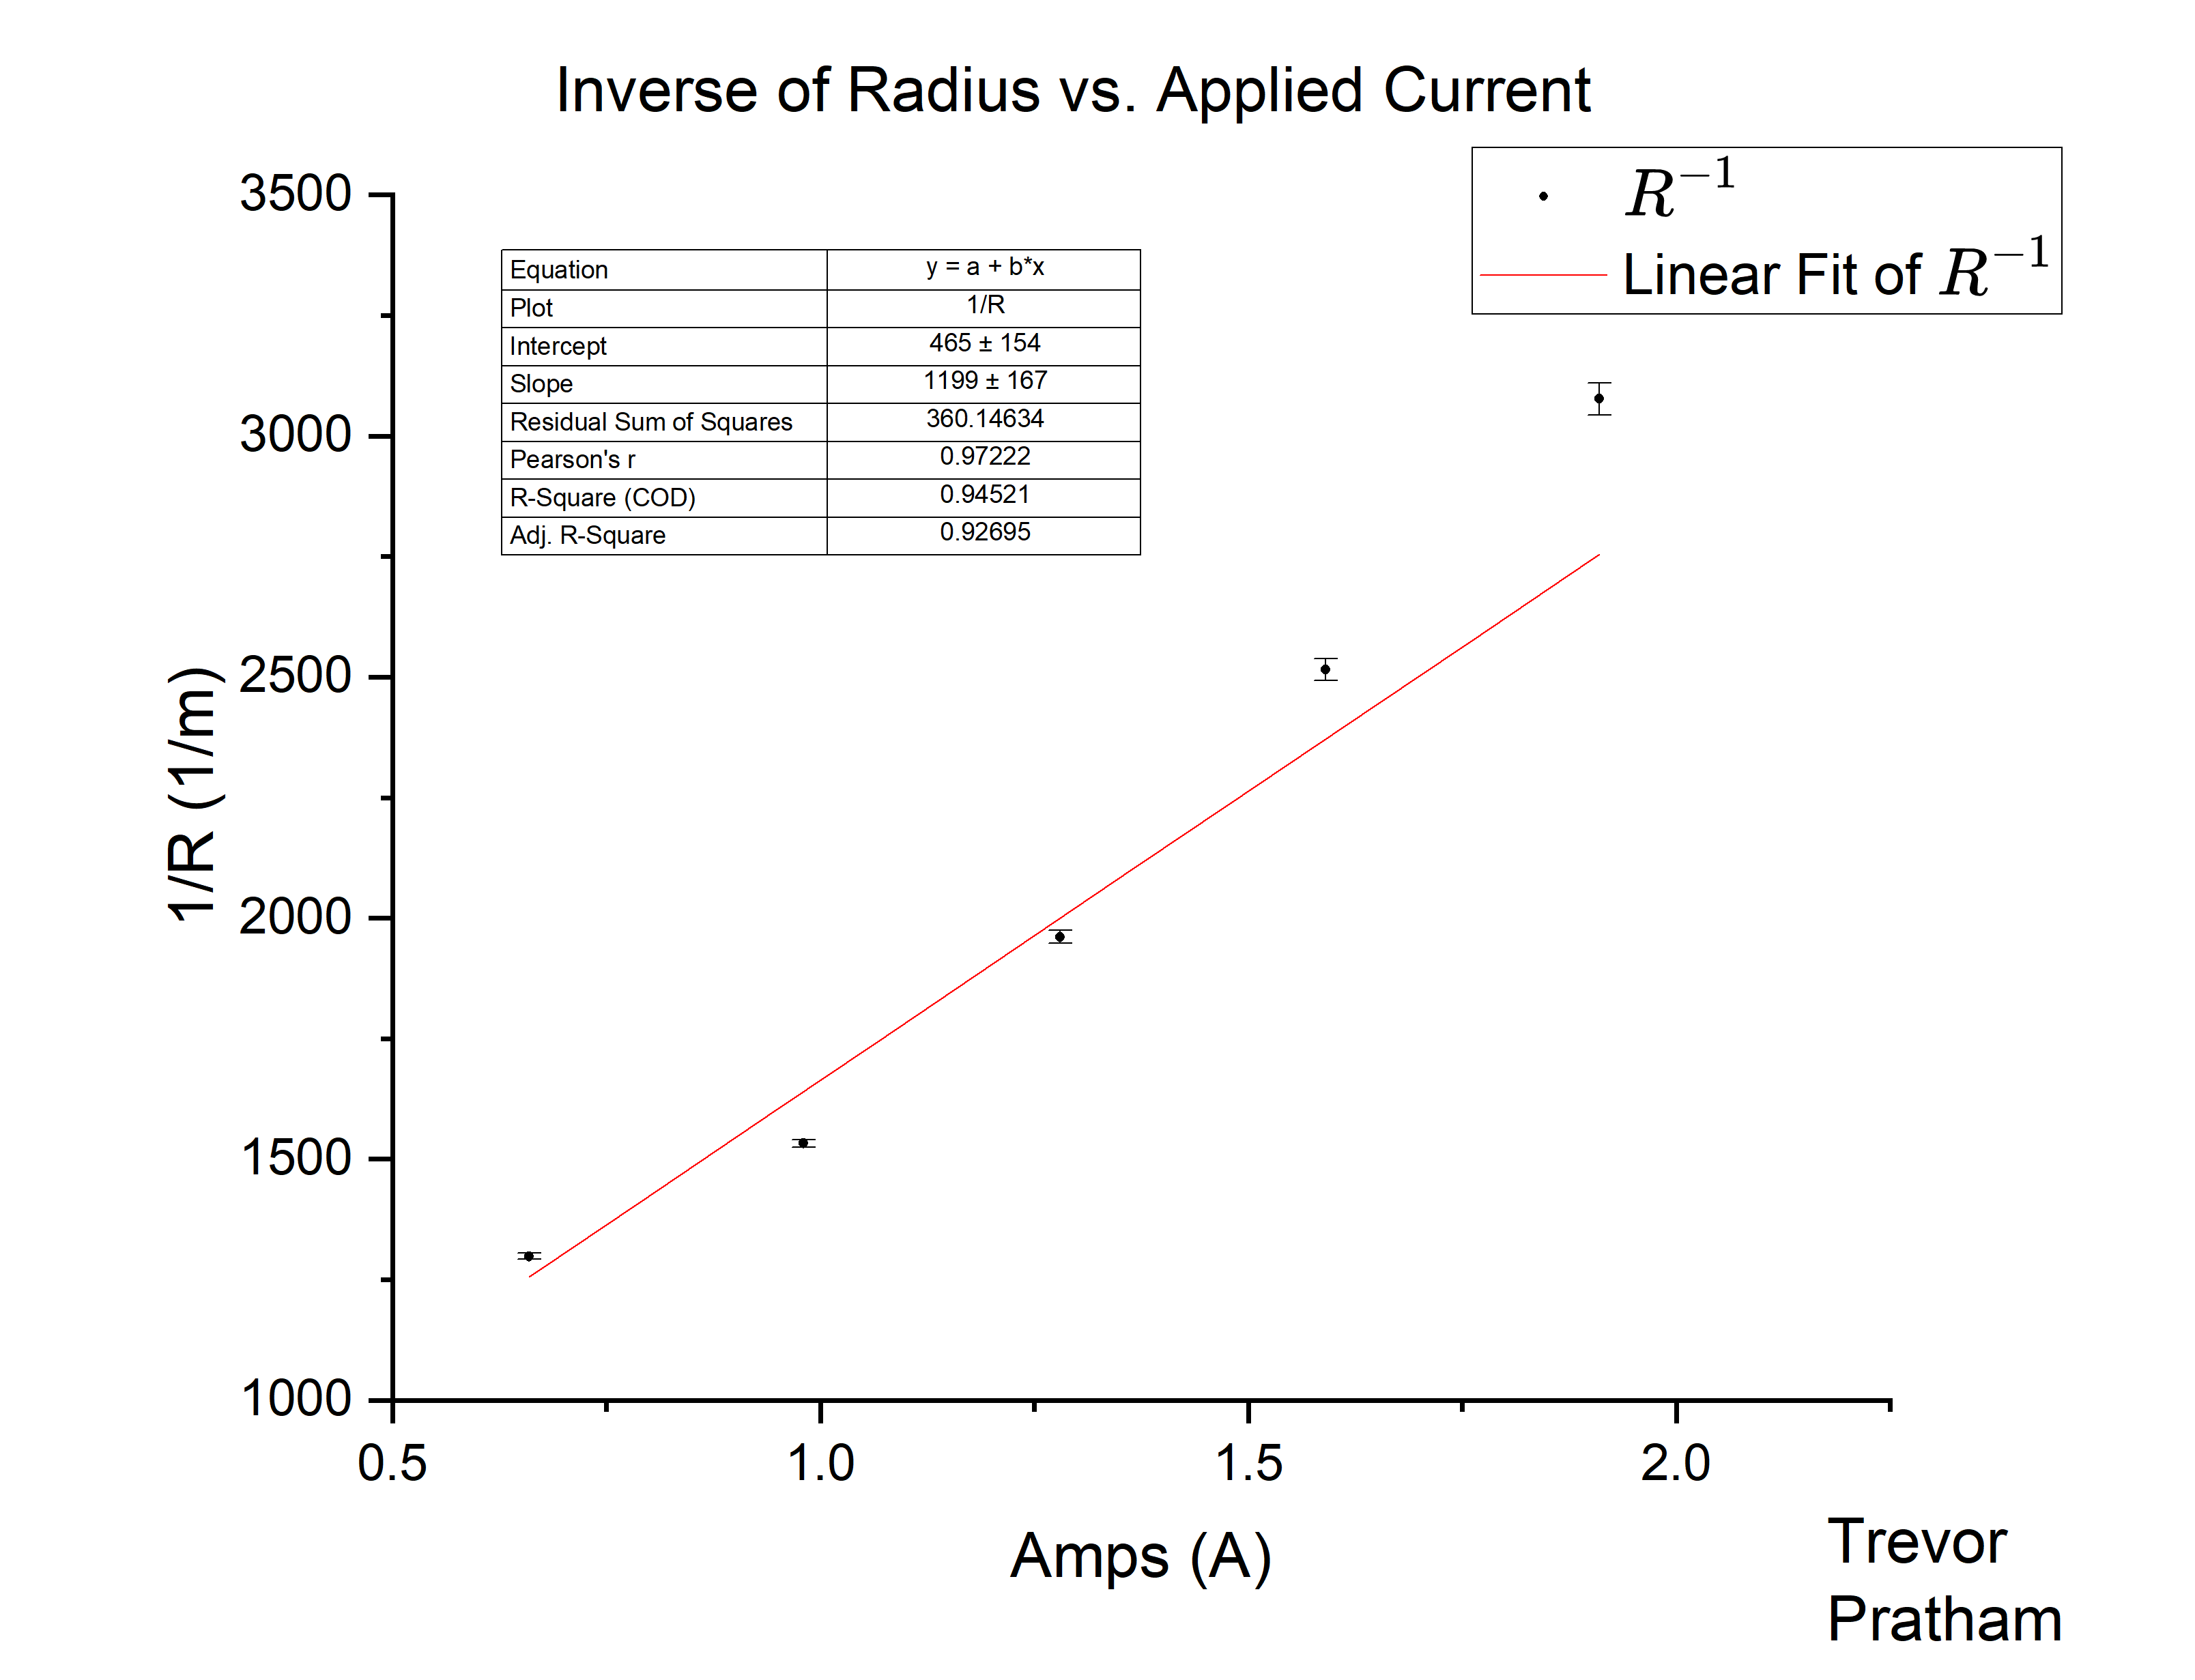
\includegraphics[width=0.7\textwidth]{figures/EOM_Fix_Voltage.png}
        \caption{Inverse of radius $\frac{1}{R}$ vs. applied current $A$. 1/R is calculated as 1 over the Average Radius values reported in Table \ref{t:FixV}.}
        \label{f:FixV}
    \end{subfigure}
\end{figure}

\clearpage

\subsection{Fixed Amps Data and Figures}

\begin{table}[h]
    \centering
    \begin{tabular}{|c|c|c|c|}
        \hline
        Voltage & Trevor's D (cm) & Pratham's D (cm) & Average Radius (m) \\ 
        \hline
        84 & 10.4 $\pm$ 0.1 & 10.3 $\pm$ 0.1 & 5.175E-4 $\pm$ 3.5E-6 \\ 
        113 & 11.8 $\pm$ 0.1 & 12.5 $\pm$ 0.1 & 6.075E-4 $\pm$ 3.5E-6 \\ 
        139 & 14.4 $\pm$ 0.1 & 13.7 $\pm$ 0.1 & 7.025E-4 $\pm$ 3.5E-6 \\ 
        168 & 15.2 $\pm$ 0.1 & 14.8 $\pm$ 0.1 & 7.500E-4 $\pm$ 3.5E-6 \\
        197 & 15.8 $\pm$ 0.1 & 15.5 $\pm$ 0.1 & 7.825E-4 $\pm$ 3.5E-6 \\
        \hline
    \end{tabular}
    \caption{Fixed Amps at $A = 1.02\pm0.01 A$, with steps of voltage from a minimum Voltage of $84V$ and a maximum of $197V$. Trevor's and Pratham's D refers to their measured diameter values, respectively. The Average Radius Values and Uncertainties here are identical to the values calculated Table \ref{t:FixV}. See the next section for uncertainty discussions.}
    \label{t:FixA}
\end{table}

\begin{figure} [h]
    \begin{subfigure}
        \centering
        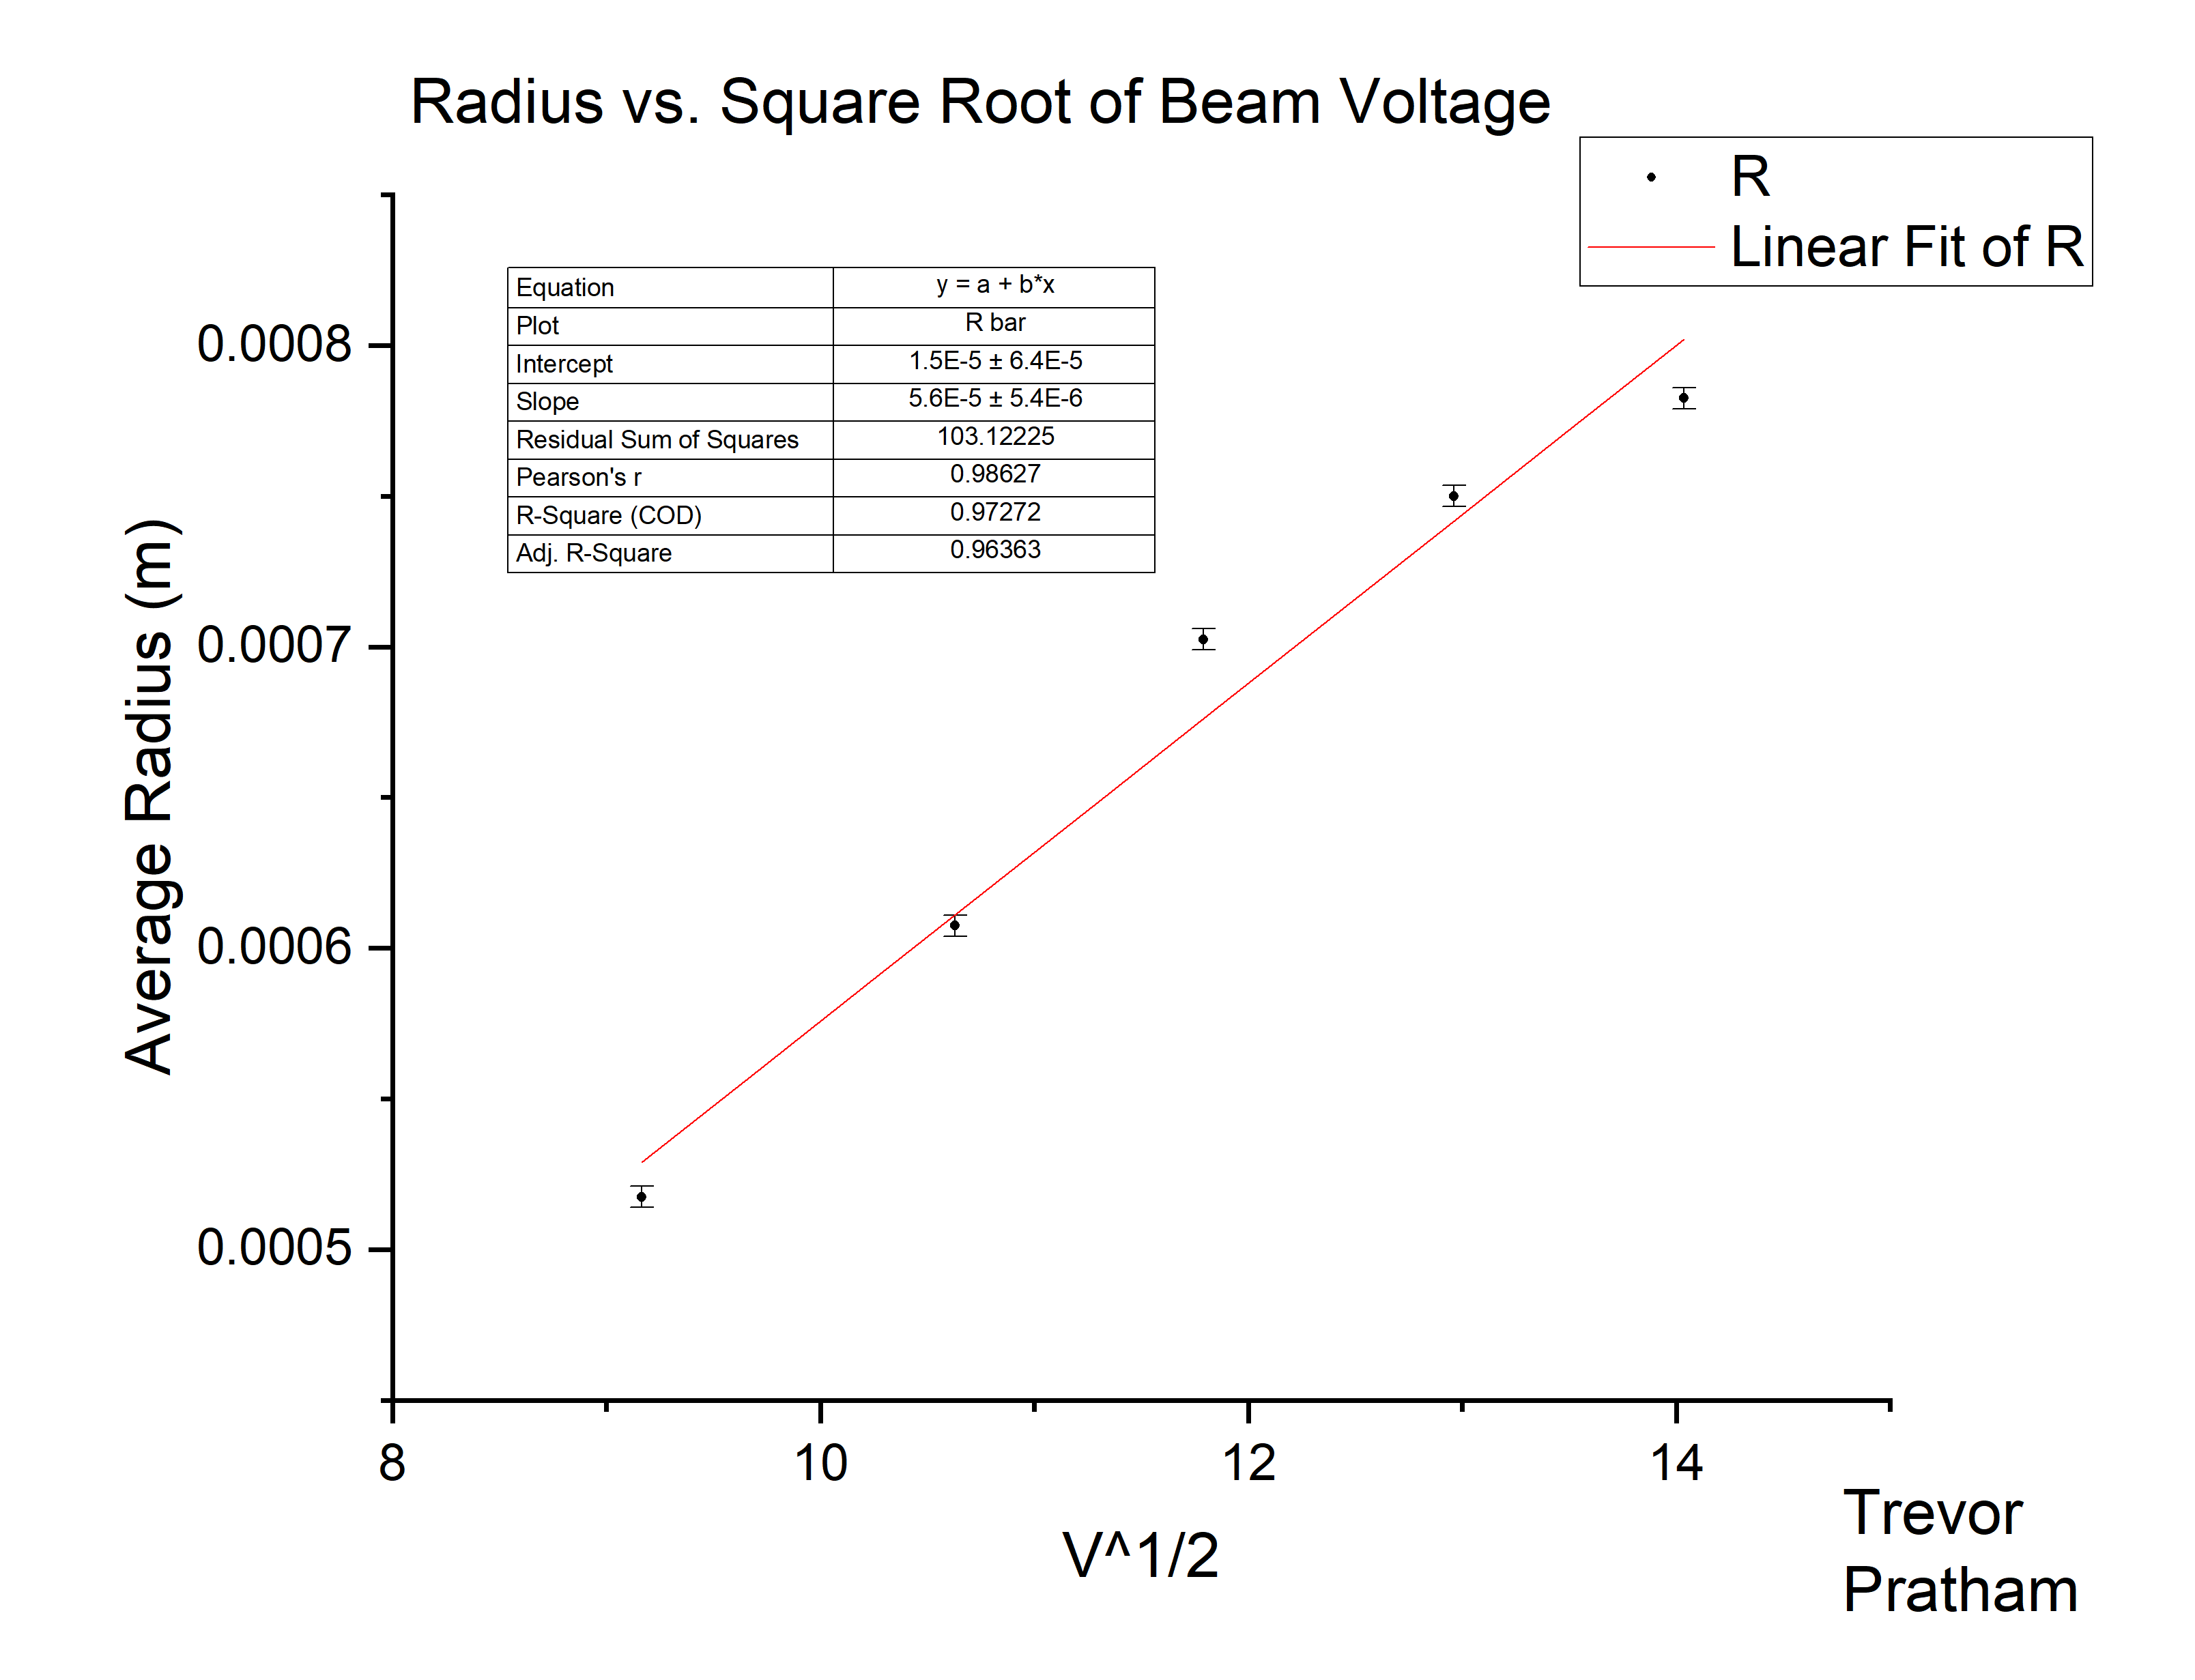
\includegraphics[width=0.7\textwidth]{figures/EOM_Fix_Amps.png}
        \caption{Radius $R$ vs. applied beam voltage $V$}
        \label{f:FixA}
    \end{subfigure}
\end{figure}

\clearpage

\section{Other Calculations} \label{sec:ERROR}
\subsection{Average Radius Error Propagation} \label{sec:RadiusErr}

\begin{align}
	\bar{R} =& \frac{1}{2}\cdot\frac{D_T + D_P}{2}\cdot\frac{1 m}{100 cm} = \frac{1}{400}\cdot(D_T + D_P)\ m \label{e:R_calculation} 	
\end{align}

$D_T$ and $D_P$ refer to diameter measurements taken by Trevor and Pratham, respectively.

\begin{align}
	\delta_{\bar{R}} =& \sqrt{\delta_{\bar{R}_{D_T}}^2 + \delta_{\bar{R}_{D_P}}^2} && \text{errors present only in }D_T \text{ and }D_P \label{e:R_bar_err_exp}
\end{align}

\begin{align}
	\delta_{\bar{R}_{D_T}} =& \left( \frac{\partial \bar{R}}{\partial D_T} \right)\cdot\delta_{D_T} = \frac{1}{400}\cdot\delta_{D_T} && \text{use }\delta_{D_T}=0.001\text{ m -- from measurements} \label{e:R_err_Dt} \\
	=& \frac{1}{400}\cdot0.001=2.5\times10^{-6} m \notag
\end{align}

\begin{align}
	\delta_{\bar{R}_{D_T}} =& \left( \frac{\partial \bar{R}}{\partial D_P} \right)\cdot\delta_{D_P} = \frac{1}{400}\cdot\delta_{D_P} && \text{use }\delta_{D_P}=0.001\text{ m -- from measurements} \label{e:R_err_Dp} \\
	=& \frac{1}{400}\cdot0.001=2.5\times10^{-6} m \notag
\end{align}

\begin{align*}
	\therefore \delta_{\bar{R}} =& \sqrt{(2.5\times10^{-6}m)^2+ (2.5\times10^{-6}m)^2} = 3.5\times10^{-6} m 
\end{align*}

\begin{equation}
	\delta_{\bar{R}} = 3.5\times10^{-6} m
	\label{v:R_bar_err}
\end{equation}

\subsection{Error Propagation in 1/R} \label{sec:InvRadiusError}

\begin{align}
	\frac{1}{\bar{R}}=& \frac{1}{R} && \text{Used for determining }\alpha \notag \\
	\delta_{\frac{1}{\bar{R}}} =& \delta_{\frac{1}{\bar{R}}_{\bar{R}}} && \text{No need for adding in quadrature, only once source of error} \notag \\
	\delta_{\frac{1}{\bar{R}}_{\bar{R}}} =& \abs{\paren{\frac{\partial \frac{1}{\bar{R}}}{\partial \bar{R}}}\cdot\delta_{\bar{R}}} && \text{Derivative method for error propagation} \label{e:R_inv_err} \\
	=& \frac{\delta_{\bar{R}}}{\bar{R}^2} && \text{Simple single-variable derivative} \notag
\end{align}

This expression was used in determining the errors presented in Table \ref{t:FixV}, but calculations are omitted here to prevent redundancy. To calculate, use $\delta_{\bar{R}}=3.5\times10^{-6} m$, as calculated in the above subsection.

\begin{equation}
	\delta_{\frac{1}{\bar{R}}}=\frac{\delta_{\bar{R}}}{\bar{R}^2}
	\label{e:R_bar_inverse_err}
\end{equation}

\clearpage

\subsection{Error Propagation in Dependence on Current} \label{sec:FixedVoltageErr}

\begin{equation}
	\alpha = \frac{8\mu_0N}{5r}\sqrt{\frac{e/m}{10V}}\
	\quad \Rightarrow \quad
	\frac{e}{m}=\paren{\frac{5r\alpha}{8\mu_0N}}^2\cdot(10V)
	\quad \text{Errors propagated in }\alpha, V, r 
	\label{e:em_derive_FixV}
\end{equation}

\begin{align}
	\delta_\frac{e}{m}=\sqrt{\paren{\delta_{\frac{e}{m}_\alpha}}^2+\paren{\delta_{\frac{e}{m}_V}}^2+\paren{\delta_{\frac{e}{m}_r}}^2} \qquad \text{General Error Equation} \label{e:FixV_err}
\end{align}

Calculate the error in $\frac{e}{m}$ due to $\alpha$ as:

\begin{align}
	\delta_{\frac{e}{m}_\alpha} = \paren{\frac{\partial \frac{e}{m}}{\partial \alpha}}\cdot\delta_\alpha =& \paren{20\paren{\frac{5}{8\mu_0N}}^2(r\alpha^2)V}\cdot\delta_\alpha \label{e:FixV_err_alpha} \\
	=& \paren{20\paren{\frac{5}{8\cdot4\pi\times10^{-7}\cdot130}}^2(0.158\cdot1199^2)\cdot104}\cdot167 \notag \\
	=& 1.15\times10^{18} \frac{C}{Kg} \notag
\end{align}

Calculate the error in $\frac{e}{m}$ due to $V$ as:

\begin{align}
	\delta_{\frac{e}{m}_V} = \paren{\frac{\partial \frac{e}{m}}{\partial V}}\cdot\delta_V =& \paren{10\paren{\frac{5}{8\mu_0N}}^2(r^2\alpha^2)}\cdot \delta_V \label{e:FixV_err_V} \\
	=& \paren{10\paren{\frac{5}{8\cdot4\pi\times10^{-7}\cdot130}}^2(0.158^2\cdot1199^2)}\cdot1 \notag \\
	=& 5.25\times10^{12} \frac{C}{Kg} \notag
\end{align}

Calculate the error in $\frac{e}{m}$ due to $r$ as:

\begin{align}
	\delta_{\frac{e}{m}_r} = \paren{\frac{\partial \frac{e}{m}}{\partial r}}\cdot\delta_r =& \paren{20\paren{\frac{5}{8\mu_0N}}^2(r^2\alpha)V}\cdot \delta_r \label{e:FixV_err_r} \\
	=& \paren{20\paren{\frac{5}{8\cdot4\pi\times10^{-7}\cdot130}}^2(0.158^2\cdot1199)\cdot104}\cdot0.005 \notag \\
	=& 4.38\times10^7 \frac{C}{Kg} \notag
\end{align}

\begin{align}
	\delta_\frac{e}{m} =& \sqrt{(1.15\times10^{18})^2+(5.25\times10^{12})^2+(4.38\times10^7)^2} && \text{Substitute Values} \notag \\
	=& 1.15\times10^{18} \frac{C}{Kg} \label{v:FixV_err}
\end{align}

\clearpage

\subsection{Error Propagation in Dependence on Voltage} \label{sec:FixedAmpsErr}

\begin{align}
	\beta = \frac{5r}{8\mu_0N I_c}\sqrt{\frac{10}{e/m}}
	\quad \Rightarrow \quad
	\frac{e}{m}=10\paren{\frac{8\mu_0N I_C\beta}{5r}}^{-2}
	\quad \text{Errors propagated in }\beta, I_c, r
	\label{e:em_derive_FixA}
\end{align}

\begin{align}
	\delta_\frac{e}{m}=&\sqrt{\paren{\delta_{\frac{e}{m}_\beta}}^2+\paren{\delta_{\frac{e}{m}_{I_c}}}^2+\paren{\delta_{\frac{e}{m}_r}}^2} \qquad \text{General Error Equation} \label{e:FixA_err}
\end{align}

Calculate the error in $\frac{e}{m}$ due to $\beta$ as:

\begin{align}
	\delta_{\frac{e}{m}_\beta} = \abs{\paren{\frac{\partial \frac{e}{m}}{\partial \beta}}\cdot\delta_\beta} =& \paren{\paren{\frac{8\mu_0N}{5}}^{-2}\cdot\paren{\frac{20r^2}{\beta^3I_c^2}}}\cdot\delta_\beta \label{e:FixA_err_beta} \\
	=& \paren{\paren{\frac{8\cdot4\pi\times10^{-7}*130}{5}}^{-2}\cdot\paren{\frac{20(0.158)^2}{(5.6\times10^{-5})^3(1.02)^2}}}\cdot(5.4\times10^{-6}) \notag \\
	=& 2.16\times10^{14} \frac{C}{Kg} \notag
\end{align}

Calculate the error in $\frac{e}{m}$ due to $I_c$ as:

\begin{align}
	\delta_{\frac{e}{m}_{I_c}} = \abs{\paren{\frac{\partial \frac{e}{m}}{\partial I_c}}\cdot\delta_{I_c}} =& \paren{\paren{\frac{8\mu_0N}{5}}^{-2}\cdot\paren{\frac{20r^2}{\beta^2I_c^3}}}\cdot \delta_{I_c} \label{e:FixA_err_Ic} \\
	=& \paren{\paren{\frac{8\cdot4\pi\times10^{-7}*130}{5}}^{-2}\cdot\paren{\frac{20(0.158)^2}{(5.6\times10^{-5})^2(1.02)^3}}}\cdot0.01 \notag \\
	=& 2.20\times10^{13} \frac{C}{Kg} \notag
\end{align}

Calculate the error in $\frac{e}{m}$ due to $r$ as:

\begin{align}
	\delta_{\frac{e}{m}_r} = \abs{\paren{\frac{\partial \frac{e}{m}}{\partial r}}\cdot\delta_r} =& \paren{\paren{\frac{8\mu_0N}{5}}^{-2}\cdot\paren{\frac{20r}{\beta^2I_c^2}}}\cdot \delta_r \label{e:FixA_err_r} \\
	=& \paren{\paren{\frac{8\cdot4\pi\times10^{-7}*130}{5}}^{-2}\cdot\paren{\frac{20(0.158)}{(5.6\times10^{-5})^2(1.02)^2}}}\cdot0.005 \notag \\
	=& 1.42\times10^{14} \frac{C}{Kg} \notag
\end{align}

\begin{align}
	\delta_\frac{e}{m} =& \sqrt{(2.16\times10^{14})^2+(2.20\times10^{13})^2+(1.42\times10^{14})^2} && \text{Substitute Values} \notag \\
	=& 2.59\times10^{14} \frac{C}{Kg} \label{v:FixA_err}
\end{align}

\end{document}
